\chapter{RAUFlow}
\label{Capítulo 5}

% **************************** Define Graphics Path **************************
\ifpdf
    \graphicspath{{Chapter5/Figs/Raster/}{Chapter5/Figs/PDF/}{Chapter5/Figs/}}
\else
    \graphicspath{{Chapter5/Figs/Vector/}{Chapter5/Figs/}}
\fi

En cap\'itulos anteriores se han detallado las caracter\'isticas m\'as importantes del prototipo así como sus componentes. Resta detallar entonces el dise\~no e implementaci\'on de RAUFlow la aplicaci\'on encargada de implementar el plano de control en el prototipo. 

En el presente cap\'itulo se propone un an\'alisis de RAUFlow siguiendo un proceso de dise\~no tradicional de Ingenier\'ia de Software dividido en cuatro etapas. Una primera etapa de an\'alisis de requerimientos, una segunda etapa de relevamiento de casos de uso, una tercera etapa de dise\~no del modelo de datos y finalmente una cuarta etapa destinada al dise\~no general de la arquitectura. Ademas se presentan los aspectos m\'as importantes relacionados a la implementaci\'on de RAUFlow como por ejemplo las implementaciones del algoritmo de ruteo y del algoritmo de distribución de etiquetas, como se implementa clasificaci\'on de tr\'afico y como se puede implementar QoS entre otros detalles. 

\section[An\'alisi de requerimientos]{An\'alisis de requerimientos}
\label{section5.1}

Anteriormente en la sección ~\ref{3.1} se definieron los requerimientos relevados para el prototipo de la RAU2. De ellos y de un trabajo de an\'alisis sobre la realidad modelada se desprende la siguiente tabla de requerimientos para RauFlow:

\clearpage
\begin{table}[Htl]\centering
\begin{tabularx}{\textwidth}{|>{\setlength\hsize{1.0\hsize}\setlength\linewidth{\hsize}}X|}
\hline
Requerimientos Funcionales\\ \hline
\hline
\begin{itemize}
\item El Sistema debe de proveer la facilidad para obtener la informaci\'on asociada a cada nodo de la red, permitiendo a su vez agregar informaci\'on que facilite la identificaci\'on del mismo para un usuario.
\item El Sistema debe proveer la facilidad para agregar, modificar y eliminar servicios de redes virtuales. 
%En particular al trabajar con redes virtuales y sus datos, se debe soportar el manejo de datos como la numeraci\'on IP del tr\'afico asociado a una red virtual, informaci\'on de capa de transporte, entre otros.
\item El Sistema debe proveer la facilidad para obtener toda la informaci\'on relevante a un servicio de red privada.
\item El Sistema debe permitir visualizar los caminos constru\'idos para encaminar el tr\'afico de una red virtual en particular, a trav\'es de la red del protot\'ipo.
\item El Sistema debe proveer la facilidad para visualizar el estado de las tablas de flujos asociadas a cualquier nodo de la red del protot\'ipo.
\end{itemize}\\
\hline
\end{tabularx}
\end{table}

\begin{table}[Htl]\centering
\begin{tabularx}{\textwidth}{|>{\setlength\hsize{1.0\hsize}\setlength\linewidth{\hsize}}X|}
\hline
Requerimientos no Funcionales\\ \hline
\hline
\begin{itemize}
\item Se debe utilizar siempre que sea posible herramientas de software libre y c\'odigo abierto.
\end{itemize}\\
\hline
\end{tabularx}
\end{table}

Teniendo en cuenta la descripci\'on del problema y los requerimientos anteriores, se procede con el modelado de la realidad. Los resultados obtenidos se presentan en la siguiente secci\'on.

%Teniendo en cuenta los requerimientos anteriores, se procede con el relevamiento de los casos de uso. Los resultados obtenidos se presentan en la siguiente secci\'on.

\section[Modelado de la realidad]{Modelado de la realidad}

Para la representaci\'on de la realidad se utiliza el paradigma de orientaci\'on a objetos. De esta forma el modelo de datos queda representado a través del siguiente diagrama de clases de diseño(ver ver figura ~\ref{fig:ModeloDeDatos}).

En el mismo se destacan en color amarillo las clases utilizadas para representar la topolog\'ia de red y sus elementos(Nodos, Interfaces y Enlaces). Cabe destacar sobre estas tres clases que en la representaci\'on asumida se busca modelar la topolog\'ia como un multigrafo dirigido. Esto se debe a que:

\begin{enumerate}
\item Tradicionalmente se utilizan grafos para el modelado de una topolog\'ia de red, siendo una representaci\'on sencilla y clara.

\item En \textbf{mpls} un camino o mejor llamado LSP tiene sentido, permitiendo por ejemplo asegurar un valor de ancho de banda en un enlace para un sentido y un valor diferente para el otro. Adem\'as permite establecer caminos diferentes para el tr\'afico en un sentido y en otro, priorizando por ejemplo el tr\'afico  en uno de los sentidos al utilizar el mejor camino. Utilizando grafos dirigidos puede modelarse este comportamiento.

\item En la pr\'actica nada impide que dos equipos o nodos est\'en conectados por m\'as de un enlace. De hecho este escenario es bastante beneficioso para asegurar conectividad ante la falla de enlaces. Utilizando multigrafos este escenario es modelado de forma clara.
  
\end{enumerate}

\begin{figure}[ht!] 
\centering    
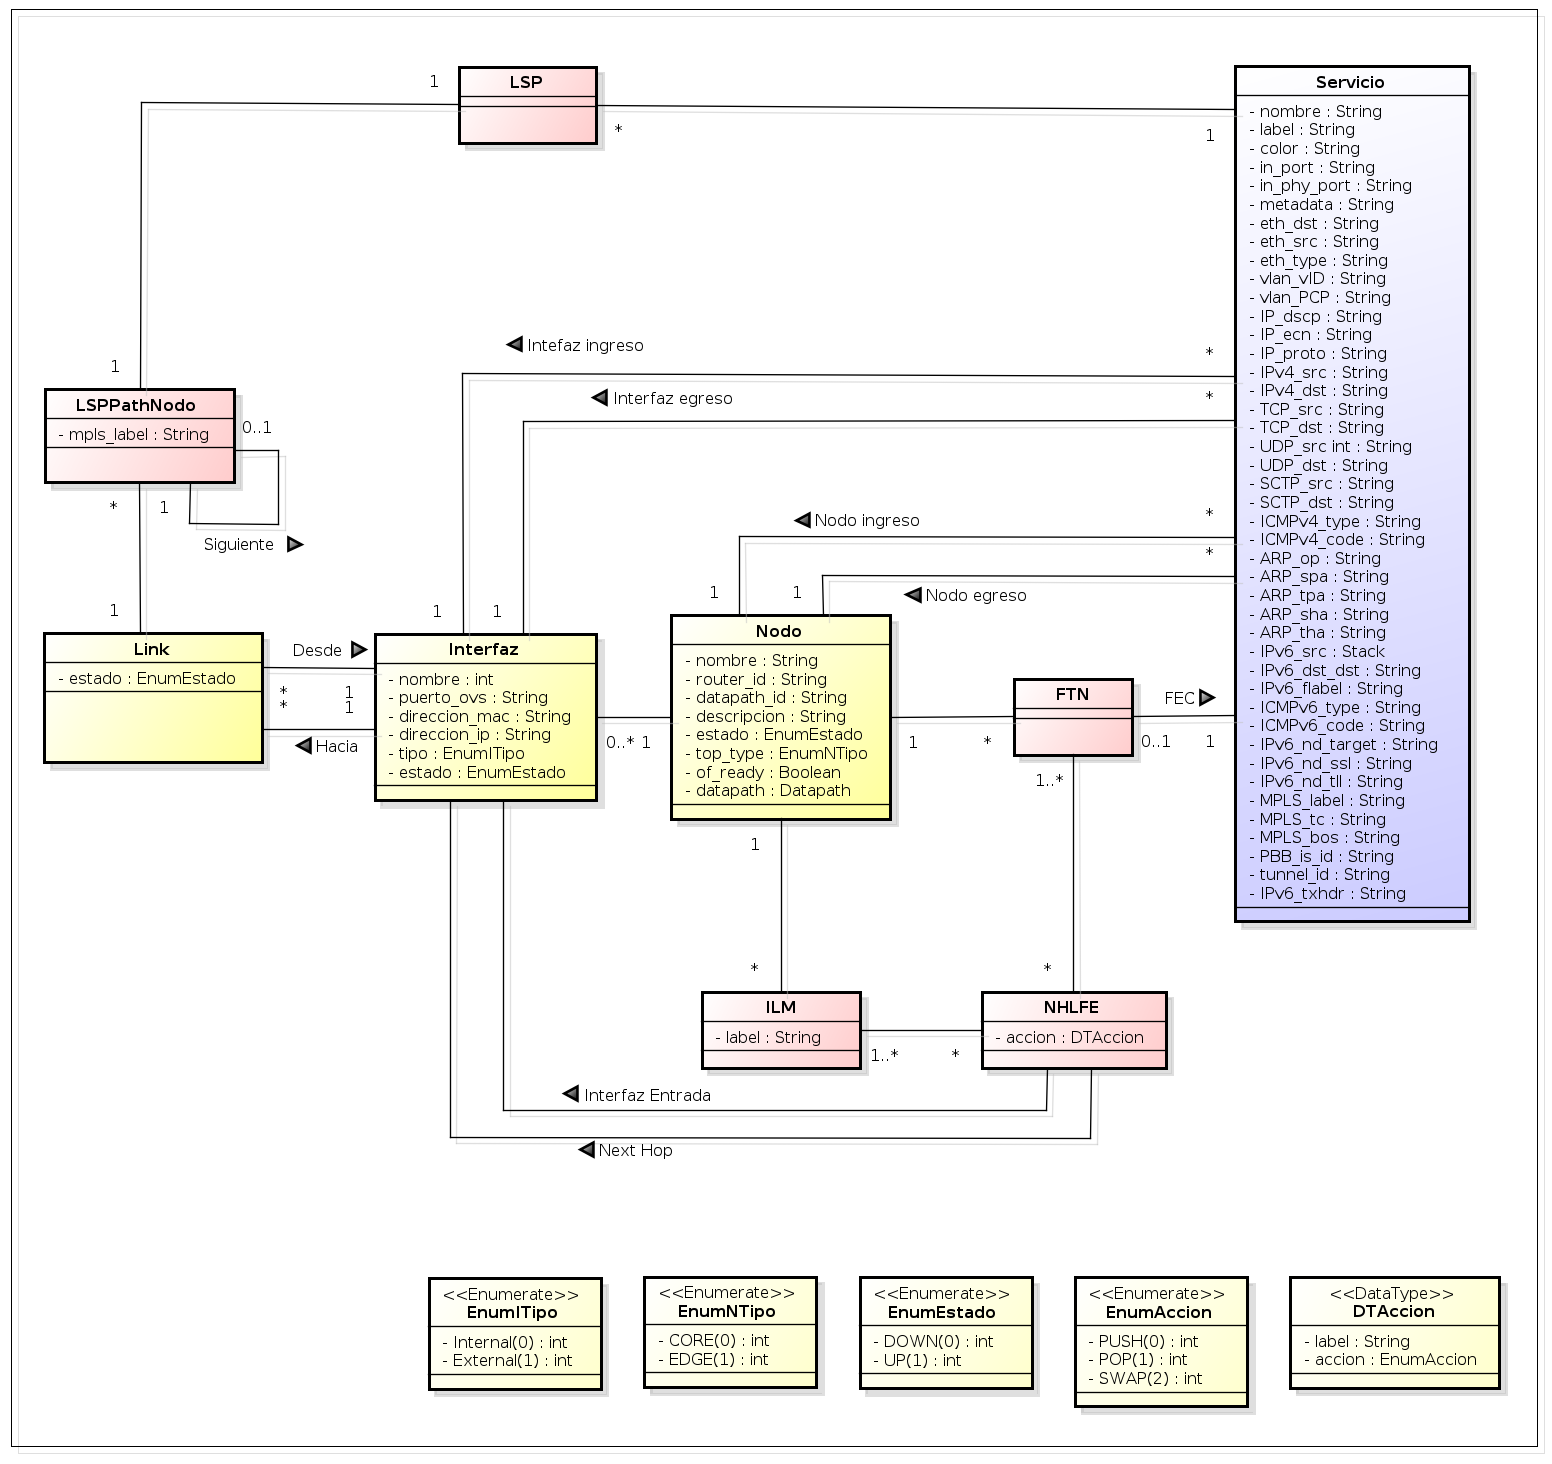
\includegraphics[width=1\textwidth]{DiagramaClases}
\caption[Modelo de datos]{Modelo de datos}
\label{fig:ModeloDeDatos}
\end{figure}

\newpage
En un mulrigrafo dirigido se tienen nodos y aristas con sentido. Cada nodo de la red puede ser representado por un nodo del grafo y cada enlace entre un par de nodos con dos aristas(una arista para cada sentido del enlace).

En el modelo se tiene adem\'as el concepto de Interfaz de dispositivo. Este concepto re-define la noción de adyacencia entre dos nodos en el grafo de la siguiente forma: existe una arista para un par de nodos si cada uno de ellos esta asociado a una instancia de la clase Interfaz y existe una instancia de la clase Link asociada a ambas interfaces mediante las relaciones “Desde” y “Hacia”; indicando adem\'as estas el sentido del dicho Link.

Cabe destacar que en el modelo la clase Nodo representa solamente dispositivos de capa 3. Esto quiere decir que dispositivos de capa 2 como switches no son contemplados. Sin embargo no se asume que el nodo este f\'isicamente implementado por RAU-Switch, con lo que se permite modelar nodos iplementados en base a otro tipo de dispositivos.\\

Por otro lado en rosado se destacan las clases utilizadas para representar los principales conceptos de \textbf{mpls} como las tablas FTN, ILM, NHLFE y el concepto de LSP. Si bien esta \'ultima clase no tiene atributos asociados en esta versi\'on del modelo de datos, eventualmente tiene sentido en un futuro que se puedan asociar atributos del camino como el m\'aximo ancho de banda disponible y algunas otras propiedades orientadas a funcionalidades de QoS por ejemplo.\\

Finalmente en azul se destaca el concepto Servicio con el cual se busca representar un servicio de red privada virtual. En particular cada instancia de Servicio representa una red privada punto a punto entre dos nodos en el prototipo; por ello esta clase tiene asociados los atributos nodo de ingreso y nodo de egreso. Adem\'as se asume que por cada nodo de borde se tiene a lo sumo una \'unica red privada conectada directamente a cada interfaz. Por ello un servicio queda determinado por los pares <nodo, intefaz> origen y <nodo, interfaz> destino. 

Luego una red privada multipunto puede construirse por ejemplo definiendo servicios punto a punto para cada par de nodos involucrados.

Esta clase también tiene asociados atributos con los cuales se implementa clasificaci\'on de tr\'afico; m\'as adelante en este cap\'itulo se detallan este y otros aspectos asociados a la implementaci\'on de esta clase.\\

%Cabe destacar que por simplicidad no se representa el concepto VPN en el modelo puesto que el foco de la aplicación esta puesto en el desarrollo de los algoritmos y funcionalidades, y no en un modelado exhaustivo de la realidad. Sin embargo este concepto como muchos otros pueden ser incorporados fácilmente en un futuro.\\

Teniendo en cuenta los requerimientos mencionados, y el modelado de la realidad presentado, se procede con el relevamiento de los casos de uso. Los resultados obtenidos se presentan en la siguiente secci\'on.

\section[Relevamiento de casos de uso]{Relevamiento de casos de uso}
\label{section5.3}

La lista de casos de uso presentada a continuaci\'on se corresponde con un conjunto de funcionalidades b\'asicas, que permiten explorar el potencial del enfoque SDN aplicado a la implementaci\'on de un prototipo para la RAU2.\\ 

\begin{itemize}
\item \textbf{CU1. Listar Servicios}: Devuelve un listado con los servicios existentes en el sistema, mostrando para cada uno la informaci\'on b\'asica asociada.

\item \textbf{CU2. Seleccionar Servicio}: Selecciona un Servicio de una lista de servicios (CU2. Listar servicios).

\item \textbf{CU3. Ver Servicio}: Devuelve la informaci\'on asociada al Servicio.

\item \textbf{CU4. Modificar Servicio}: Modifica una instancia de Servicio, actualizando los atributos seleccionados por el usuario con los valores ingresados.
 								
\item \textbf{CU5. Eliminar Servicio}: Elimina un Servicio existente en el sistema.

\item \textbf{CU6. Agregar Servicio}: Crea un nuevo servicio de red privada en el sistema, con la inormaci\'on de nodos y sus respectivas interfaces a las que las subredes esta\'an directamente conectadas con la red del prototipo, ingresada. Adem\'as solicita para cada servicio los datos utilizados para la clasificaci\'on del tr\'afico asociado al servicio. 

\item \textbf{CU7. Ver Topolog\'ia}: Muestra la topolog\'ia de red mediante una representaci\'on gr\'afica.

\item \textbf{CU.8 Filtrar Lsps}: Superpone en la representaci\'on gr\'afica de la red (CU7.Ver Topolog\'ia), un conjunto de LSPs seleccionados.

\item \textbf{CU9. Seleccionar Nodo}: Selecciona un nodo de una lista de Nodos (CU7. Ver Topolog\'ia).

\item \textbf{CU10. Ver informaci\'on b\'asica Nodo}: Despliega la informaci\'on asociada al nodo seleccionado de la topolog\'ia (CU9. Seleccionar Nodo).

\item \textbf{CU11. Ver tabla de Flujos Nodo}: Muestra la inormaci\'on de la tabla de flujos OpenFlow asociada al nodo seleccionado (CU9. Seleccionar Nodo).

\item \textbf{CU12. Ver tablas MPLS}: Muestra la informaci\'on asociada a las tablas FTN, ILM y NHLFE asociadas al nodo seleccionado (CU9. Seleccionar Nodo).

\item \textbf{CU13. Editar Informaci\'on extra Nodo}: Permite ingresar informaci\'on adicional sobre un Nodo como Nombre, si es nodo de interno o de borde por ejemplo.

\item \textbf{CU14. Editar Informaci\'on extra Interfaz}: Ingresa informaci\'on adicional sobre la interfaz de un nodo seleccionado (CU9. Seleccionar Nodo). Por ejemplo si la interfaz es interna o externa.
\end{itemize}

En la figura \ref{fig:CasosDeUso} se representan las dependencias existentes entre los casos de uso mencionados anteriormente.\\

\begin{figure}[ht!] 
\centering    
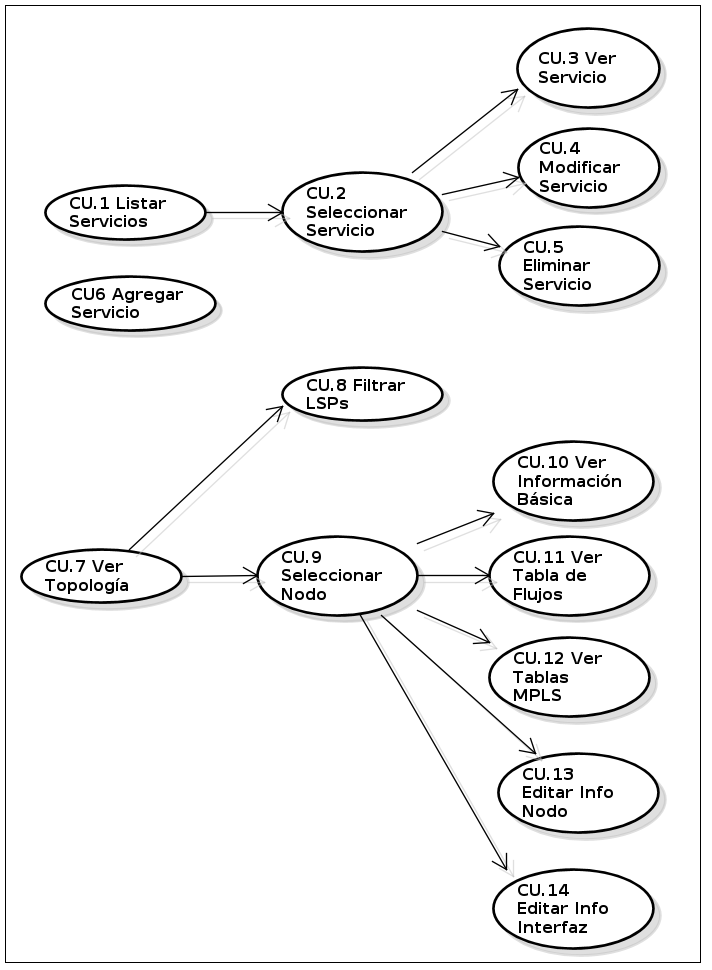
\includegraphics[width=0.7\textwidth]{CasosDeUso}
\caption[Casos de Uso de RAUFlow]{Casos de Uso de RAUFlow}
\label{fig:CasosDeUso}
\end{figure}

En la siguiente secci\'on se presenta la arquitectura de la aplicaci\'on RAUFlow, detallándose las componentes m\'as importantes.

%De esta forma quedan presentados los requerimientos relevados sobre RauFlow, el modelado de la realidad, y los casos de uso relevados. Resta entonces presentar un esbozo de la arquitectura de la aplicaci\'on RauFlow, para que el lector finalmente este en condiciones de comprender el dise\~'no del prototipo en su totoalidad.

\section[Arquitectura de RauFlow]{Arquitectura de RauFlow}

%Previo a la presentación de la arquitectura de RAUFlow vale la pena dedicar un pequeño espacio de esta sección al esclarecimiento de algunos aspectos clave para el entendimiento de la arquitectura de la aplicaci\'on. 

Como se menciona en el cap\'itulo anterior, RAUFlow es el nombre dado a la aplicaci\'on encargada de implementar el plano de control en el prototipo. Sin embargo como se menciona tambi\'en en dicho cap\'itulo, la o las aplicaciones que se ejecutan en el controlador Ryu interactuan con diferentes m\'odulos y componentes como el Administrador SNMP \'o la base de datos topol\'ogica de Quagga. Por esta raz\'on tiene sentido pensar en RAUFlow como el conjunto de todas estas componentes las cuales interactuando entre ellas implementan efectivamente el plano de control.\\

Conceptualmente RAUFlow es una aplicaci\'on de gestión de red, basada en el enfoque de SDN e implementada utilizando el software de Control Ryu y el protocolo OpenFlow entre otras tecnologías principalmente. No es puramente una aplicaci\'on OpenFlow puesto que como se ha mencionado reiteradas veces utiliza un conjunto de componentes y m\'odulos independientes del ambiente del controlador Ryu.

%Con el objetivo de mantener simple y modular el dise\~no de RauFlow, se implementa en RauFlowApp solamente aquellas funcionalidades y responsabilidades asociadas al protocolo OpenFlow y sus respectivos eventos. Luego responsabilidades y funcionalidades asociadas a la realidad modelada y sus reglas de negocios, son delegadas a una capa de negocios. Ademas se tiene un conjunto de aplicaciones Ryu dise\~nadas e implementadas por terceros, las cuales se encuentran dentro del conjunto de aplicaciones que vienen con el software Ryu. M\'as adelante se explicar\'a en detalle cual es el rol que cumplen estas aplicaciones en el dise\~no de RauFlow.

%Para completar esta visi\'on general de RauFlow, se incluye en su arquitectura una interfaz de usuario gr\'afica.\\ 

%En res\'umen, el dise\~no de RauFlow se caracteriza por una arquitectura en cuatro capas: (1) capa de presentación, (2) capa de aplicaciones Ryu, (3) capa de negocios, y (4) capa de dispositivos.\\

\begin{figure}[h] 
\centering    
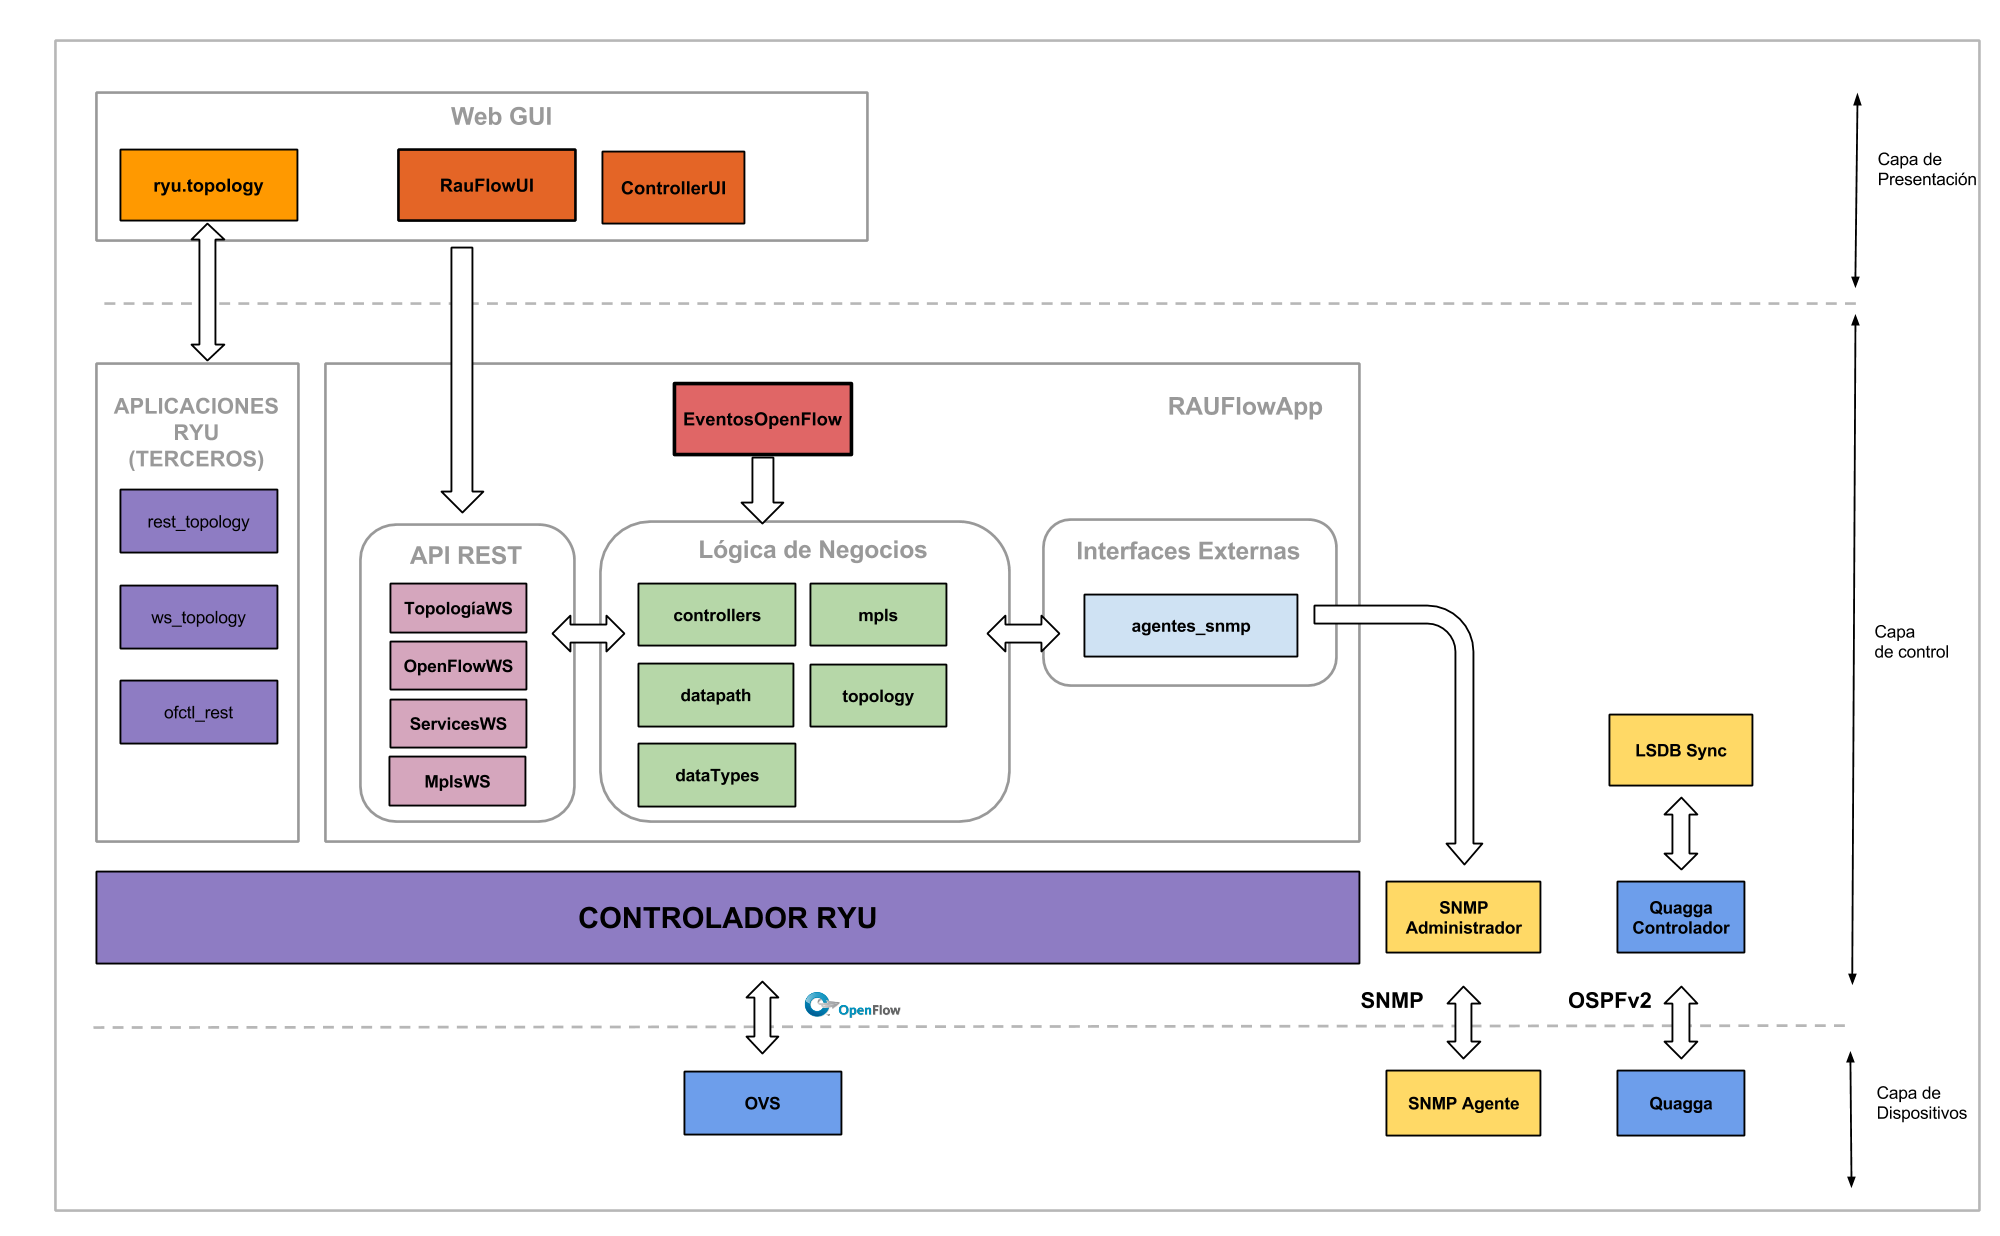
\includegraphics[width=1.0\textwidth]{Disenio_Figure4}
\caption[Vista l\'ogica]{Vista l\'ogica}
\label{fig:VistaComponentes2}
\end{figure}

Teniendo en cuenta lo anterior, la arquitectura de la aplicaci\'on (ver figura \ref{fig:VistaComponentes2}), se caracteriza por un diseño en tres capas l\'ogicas: (1) capa de presentaci\'on, (2) capa de control y (3) capa de dispositivos.\\

A continuaci\'ion se explica en detalle cada una de estas capas, as\'i como la interacci\'on entre ellas y los principales detalles de los m\'odulos que las componen.

\subsection{Capa de Presentación}
Esta capa esta destinada a proveer de funcionalidades para el acceso y manipulaci\'on de datos de la aplicaci\'on (estado de la topolog\'ia e informaci\'on asociada a servicios de redes privadas principalmente), as\'i como todas las funcionalidades especificadas como requerimientos en la secci\'on 
\ref{section5.1}.\\ 

Dentro de la capa de presentaci\'on se destacan: (1) una interfaz gr\'afica identificada en el esquema como RauFlowUI, la cual implementa cada uno de los casos de uso mencionados anteriormente en la secci\'on \ref{section5.3}, (2) ControladorUI, componente que implementa los m\'etodos de acceso entre las funcionalidades de RauFlowUI y la capa de control a trav\'es de una API Rest de Servicios enS la capa de control y (3) un m\'odulo javascript denominado \textbf{ryu.topology}.\\ 

Ryu incluye a modo de documentaci\'on un conjunto de aplicaciones muy sencillas en las que se ejemplifica el uso de las principales funcionalidades del protocolo OpenFlow. Entre estas aplicaciones se encuentra \textbf{gui\_topology}. Esta aplicaci\'on brinda una representaci\'on gr\'afica b\'asica de de las componentes topol\'ogicas en una red OpenFlow (switches, puertos y links).

Esta aplicaci\'on se basa en tres aplicaciones Ryu de la capa de control (m\'as adelante se detalla el funcionamiento de ellas cuando se explique la capa de control), una pagina web desarrollada puramente sobre HTML y un m\'odulo de javascript encargado de la manipulaci\'on de informaci\'on entre las aplicaciones Ryu y esta p\'agina mediante websockets. Este m\'odulo javascript recibe el nombre de \textbf{ryu.topology}.

En RAUFlow se combinan las componentes de la aplicaic\'on \textbf{gui\_topology} como el m\'odulo javascript \textbf{ryu.topology} y las tres aplicaciones Ryu con el resto de las componentes de la aplicaci\'on con el objetivo de mejorar la interfaz gr\'afica RAUFlowUI, brindando una representaci\'on gr\'afica del estado topol\'ogico de la red utilizando reutilizando las herramientas existentes.\\
 
A continuaci\'on se detalla la capa de control.

\subsection{Capa de Control}

La capa de control consta de tres componentes principalmente: el software de control Ryu y el conjunto de aplicaciones SDN que se ejecutan sobre este, el m\'odulo LSDBSync y finalmente el modulo Administrador SNMP.\\

 


Por un lado, la capa de control esta integrada por el software de control Ryu y cuatro aplicaciones Ryu mencionadas. por otro lado los m\'odulos LSDBSync encargado de sincronizar la informaci\'on de la Link-State-Database en la instancia de Quagga ejecutada en la PC controlador con estas aplicaciones y SNMP Administrador encargado de la comunicaci\'on con los agentes SNMP instalados en cada nodo del prototipo. 



\subsection{Aplicaciones Ryu}
Se utilizan cuatro aplicaciones Ryu en el diseño de RAUFlow.

Por un lado se tienen tres aplicaciones que vienen con el software de control, dise\~nadas para implementar una interfaz gr\'afica, consistente en un p\'agina web implementada sobre html, javascript y web sockets. Con esto Ryu permite visualizar de forma gr\'aica la red en su totalidad; estos es los dispositivos del datapath con sus interfaces y los enlaces existentes.

Con el objetivo de proveer de una representaci\'on gr\'afica del estado de la red (el estado de la topolog\'ia y sus dispositivos), se incluyen en la arquitectura de RAUFlow este conjunto de aplicaciones. bajo el nombre Aplicaciones Ryu (Terceros)


Por otro lado la cuarta apliaci\'on es desarrollada en el marco de este trabajo, conteniendo el modelado de la realidad planteado y la implementaci\'on de las funcionalidades mencionadas.\\

En esta capa se encuentran las diferentes aplicaciones Ryu utilizadas para implementar el plano de control OpenFlow. Esta compuesta por una aplicaci\'on desarrollada en este proyecto (RAUFlowApp), y tres aplicaciones desarrolladas por terceros (incluidas en las aplicaciones que vienen con el controlador).\\

Dentro de las aplicaciones Ryu, RauFlowApp es realmente la encargada de implementar el plano de control  del prototipo. Esto quiere decir, guardar informaci\'on de la realidad (servicios de redes privadas), guardar el estado de la topolog\'ia, implementar funcionalidades de QoS, ruteo din\'amico etc. 

En consecuencia el alcance de esta aplicaci\'on puede ser casi tan grande como el propio alcance de RAUFlow. Sin embargo esto redundar\'ia en una complejidad mayor en el dise\~no de la aplicaci\'on, poca mantenibilidad, calidad del c\'odigo fuente, etc. Por estas razones se decide desacoplar la mayor cantidad de informaci\'on posible relacionada a la realidad modelada, de dicha aplicaci\'on; haciendo responsable a RauFlowApp solamente por el manejo de los eventos del protocolo OpenFlow.

De esta forma se justifica la mencionada capa de Negocios. 


\subsection{Capa de Negocios}
La capa de negocios presenta tres componentes bien definidas: una componente de reglas y l\'ogica de negocios de la realidad, una API REST de servicios para el acceso y la manipulaci\'on de datos relacionados a la primera componente y una tercera componente denominada Agentes distribu\'idos.

\subsubsection{Lógica de Negocios}
La componente lógica de negocios se subdivide a su vez en diferentes m\'odulos que agrupan funcionalidades acorde a su naturaleza y responsabilidades. Vale la pena destacar a su vez que cada uno de estos m\'odulos se corresponde en la implementaci\'on con un package en la filosof\'ia de Python. Estas funcionalidades y responsabilidades se corresponden de la siguiente forma:

\begin{itemize}
\item \textbf{controller:} Este m\'odulo agrupa diferentes controladores de objetos. Actualmente contiene un \'unico controlador façade responsable de mantener el \'unico punto de acceso a la las componentes de la l\'ogica de negocios. Contiene desde la implementaci\'on de funciones para dar de alta Servicios, crear LSPs, obtener el mejor camino entre dos nodos de la red, etc.

\item \textbf{topology:} Agrupa las definiciones de objetos utilizados para representar la topolog\'ia como las clases Nodo, Interfaz y Link, así como otros conceptos de la realidad.
 
\item \textbf{mpls:} Contiene las definiciones de los conceptos FTN, ILM, NHLFE, as\'i como los conceptos de conceptos de servicio de red y LSP(Label Switched Path).

\item \textbf{dataTypes:} Mantiene representaciones reducidas de los principales objetos definidos en todos los m\'odulos de la componente de negocios para el intercambio de datos por ejemplo con la capa de presentaci\'on. 

\item \textbf{datapath:} Agrupa funcionalidades para el acceso al datapath de OpenFlow, como funciones para agregar y eliminar flujos en un switch, u obtener estad\'isticas de una tabla de flujos.
\end{itemize} 

\subsubsection{API REST de servicios}
La componente de Servicios REST, se encuentra subdividida en varios m\'odulos respondiendo al criterio utilizado para el dise\~no modular de la componente de l\'ogica de negocios. 

\subsubsection{Agentes distribuidos}
Esta componente es la encargada de interactuar con diferentes agentes y procesos instalados en cada nodo del prototipo a través de un canal de comunicación IP. Este m\'odulo de comunicaci\'on, as\'i como los diferentes agentes instalados en cada nodo, juegan un rol irreemplazable en la obtenci\'on de informaci\'on adicional sobre cada nodo; puesto que a partir del canal de comunicaci\'on OpenFlow solamente es accesible Open vSwitch y la informaci\'on contemplada por el protocolo OpenFlow.\\

Dentro de esta componente, en el diagrama se muestra un modulo denominado \textbf{managements\_ agents}. Este m\'odulo opera como una interfaz de conexi\'on entre los diferentes m\'odulos de la l\'ogica de negocios y los diferentes m\'odulos que implementan la comunicaci\'on con su respectivo agente distribu\'ido.

En la figura ~\ref{fig:VistaComponentes2} se muestran el modulo \textbf{SNMP Management}, responsable de  la comunicaci\'on con el Agente SNMP instalado en cada nodo del prototipo, con el fin de obtener la correspondencia entre n\'umeros de puerto OpenFlow y direcciones IP de cada interfaz.\\

%\subsection{Capa de Presentación}
%Dentro de la capa de presentaci\'on se destacan: (1) una interfaz gr\'afica identificada en el esquema como RauFlowUI, la cual implementa cada uno de los casos de uso mencionados anteriormente en \ref{section5.3}, (2) ControladorUI, componente que funciona como nexo entre las funcionalidades de RauFlowUI y la API Rest de Servicios y (3) \textbf{ryu.topology}. Esta \'ultima componente forma parte del conjunto de apliaciones Ryu adicionales que se incluyen en el dise\~no de RauFlow y tiene como principal funci\'on la de proveer una representaci\'on gr\'afica en tiempo real de la topolog\'ia existente en el prototipo.\\

\section[Implementaci\'on]{Implementaci\'on}

En esta secci\'on se presentan los aspectos m\'as importantes relacionados a la implementaci\'on de RauFlow. Entre ellos se destacan la estrategia utilizada para implementar clasificaci\'on de tr\'afico,  la implementaci\'on de la clase servicio, la implementaci\'on de los algoritmos de ruteo y distribución de etiquetas distribusi\'on de etiquetas, entre otros.\\

\subsection{Clasificación de tr\'afico}
En la literatura de MPLS, tradicionalmente se utiliza el concepto de FEC(fordwarding equivalence class) para distinguir a un conjunto de paquetes a ser tratados en forma similar(por ejemplo para aplicar t\'ecnicas de QoS). Este concepto se define localmente a un dispositivo, determinando la forma en que un conjunto de paquetes son tratados solamente en el mismo.

En RAUFlow se aprovecha la visi\'on global del plano de control SDN para definir una noci\'on de FEC global en una topolog\'ia de red. En esta redefinici\'on se clasifica tr\'afico solamente en el nodo de ingreso a la red del prototipo, determinándose all\'i el camino a seguir por un paquete hasta el nodo de egreso mediante el resultado obtenido en la ejecuci\'on del algoritmo de ruteo. 

%Este camino es calculado por el algoritmo de ruteo, eventualmente un algoritmo con restricciones(CSPF) en el cual se contemplan políticas de ingenieria de tr\'afico y calidad de servicios. 

Por otro lado se define un mapeo entre servicios de VPN y etiquetas mpls, permitiendo identificar el tr\'afico asociado a un servicio particular en cualquier nodo de la red. Luego a partir del valor de esta etiqueta se puede realizar un procesamiento diferencial en nodos intermedios de un LSP.\\

%Cuando un nuevo servicio de VPN es instanciado en RAUFlow, se ejecutan el algoritmo de ruteo para obtener el mejor camino dentro de la red, y el algoritmo de distribución de etiquetas para hallar el mapeo a etiquetas MPLS a conmutar por cada nodo del camino(LSP). Por como esta definido el algoritmo de distribución de etiquetas, este LSP es \'unico y permite identificar al servicio en cada salto por la etiqueta que se esta conmutando. De esta forma no es necesario clasificar estrictamente hablando el tr\'afico en cada nodo intermedio de la red, puesto que su camino esta dado una vez que ingresa a la red y es clasificado.

En relaci\'on a como se implementa clasificaci\'on de tr\'afico, en el prototipo se utilizan las tablas de flujos de Open vSwitch en conjunto con los campos del cabezal OpenFlow (matching fields) para la definici\'on de flujos. Con los matching fields de OpenFlow se define la regla de un flujo(recordar figura \ref{fig:OpenFlowArch2}) distinguiendo de este modo entre diferentes clases de tr\'afico para un procesamiento diferencial.

Dentro del cabezal OpenFlow, existen campos para la definici\'on de las reglas de un flujo, campos para la definici\'on de la acci\'on de un flujo y campos que pueden ser utilizados para la definici\'on de ambas componentes.  

Esta lista de campos varia con la versi\'on del protocolo OpenFlow y en el contexto del prototipo esta acotada a su vez por la implementaci\'on de Open vSwitch. En el ap\'endice \ref{appendix3} se muestra  la lista entera de atributos que contiene el cabezal OpenFlow para la versi\'on 1.3 y de estos la lista de atributos que son soportados por Open vSwitch y que pueden ser utilizados para la definici\'on de reglas y acciones. Ambas listas fueron constru\'idas experimentalmente trabajando con las herramientas Open vSwitch y Ryu.\\

En el prototipo, el concepto de clasificaci\'on de tr\'afico esta estrictamente ligado al concepto de servicio de red privada. En la siguiente secci\'on se explica en detalle la implementaci\'on de este concepto.
 
\subsection{Implementación de Servicio}

La clase Servicio implementa en el prototipo el concepto de servicios de red privada virtual. Como se menciona anteriormente un servicio define una clase de tr\'afico; por tanto adem\'as de la informaci\'on b\'asica que define a un servicio se tienen asociados tambi\'en todos los campos utilizados para implementar clasificaci\'on de tr\'afico(matching fields de OpenFlow).

En el prototipo se asume que por cada nodo de borde  se tiene una \'unica red privada directamente conectada a cada interfaz externa. Esto permite definir un servicio a partir de la clase de tr\'afico definida y los pares nodo-interfaz origen y nodo-interfaz destino.

Por otro lado se pdr\'ia refinar la definici\'on de servicio agregando m\'as dimensiones; una dimensi\'on bastante \'util podr\'ia ser por ejemplo tiempo. Utilizando esta dimensi\'on se podr\'ia por ejemplo definir un servicio de red privada para un rango horario determinado.

De igual forma se pueden incorporarse m\'as dimensiones orientado a brindar una mayor flexibilidad en la definici\'on de servicios, de cara a lo que podr\'ian ser diferentes requerimientos de la RAU2. 

De todos modos teniendo en cuenta el alcance del proyecto se decide dejar estas dimensiones extras como una posible l\'inea de trabajo a futuro.\\ 

%En la realidad modelada se tienen dos conceptos fundamentales asociados a un servicio de red privada virtual (VPN): (1) el concepto de clasificación de tr\'afico y (2) el concepto de calidad de servicio.\\

%En el prototipo, cuando se define un servicio se define adem\'as una clase de equivalencia de tr\'afico, en otras palabras una FEC global.



%\begin{itemize}
%\item Es un concepto global que involucra a toda la topolog\'ia
%\item Queda determinado parcialmente por la cuádrupla 
%\begin{center}
%(nodo\_ingreso, interfaz\_ingreso, nodo\_egreso, interfaz\_egreso)
%\end{center}
%\item Interesa distinguir servicios utilizando las capacidades provistas por los matching fields de OpenFlow 
%\item Esta definido temporalmente (para un rango horario espec\'ifico)[esto no se si lo ponemos]
%\end{itemize}

De esta forma la clase servicio queda determinada de la siguiente forma:\\

\begin{python}
class Service(object):

		# Atributos generales
		ID 				    # str(uuid.uuid4()) ID unico  
		name 				# Nombre del servicio para 
							# identificacion de usuarios 
							# en RAUFlow
							
		lsps				# Lista de LSPs para el servicio
		
		ingress_node		# Nodo de ingreso del servicio
							
		egress_node 		# Nodo de egreso del servicio
							
		ingress_interface 	# Interfaz de ingreso en el nodo 
							# de ingreso
							
		egress_interface 	# Interfaz de egreso en el nodo 
							# de ingreso 
        
		# Campos del cabezal OFv1.3 
		in_port			# Switch input port. 
		metadata 		# Metadata passed between tables. 
		eth_dst 		# Ethernet destination address.
		eth_src 		# Ethernet source address. 
		eth_type 		# Ethernet frame type. 
		vlan_vID 		# VLAN id. 
		vlan_PCP		# VLAN priority. 
		IP_dscp 		# IP DSCP (6 bits in ToS field). 
		IP_ecn  		# IP ECN (2 bits in ToS field). 
		IP_proto		# IP protocol. 
		IPv4_src 		# IPv4 source address. 
		IPv4_dst 		# IPv4 destination address. 
		TCP_src 		# TCP source port. 
		TCP_dst 		# TCP destination port. 
		UDP_src 		# UDP source port. 
		UDP_dst 		# UDP destination port. 
		SCTP_src 		# SCTP source port. 
		SCTP_dst 		# SCTP destination port. 
		ICMPv4_type 	# ICMP type. 
		ICMPv4_code 	# ICMP code. 
		IPv6_src 		# IPv6 source address. 
		IPv6_dst 		# IPv6 destination address. 
		ICMPv6_type 	# ICMPv6 type. 
		ICMPv6_code 	# ICMPv6 code. 
		MPLS_label 		# MPLS label. 
		MPLS_tc 		# MPLS TC. 
		
\end{python}

En RAUFlow, cuando se crea un nuevo servicio se ejecutan los algoritmos de ruteo y distribución de etiquetas par construir el menos un LSP. Luego este LSP es traducido a flujos OpenFlow que luego son instalados en cada uno de los nodos que forman parte. 

En la siguiente secci\'on se detalla el algoritmo de ruteo utilizado en RAUFlow.

\subsection{Algoritmo de ruteo}
El algoritmo de ruteo implementado parte de un algoritmo Shortest Path First(SPF) centralizado para el calculo del mejor camino entre un par de nodos en la topolog\'ia. Luego incorporando restricciones al mismo es posible llegar a un Constrained Shortest Path First(CSPF) con el cual se podr\'ia implementar funcionalidades de QoS.\\

En el desarrollo de este proyecto, por razones de tiempo solo fu\'e posible la implementaci\'on del algor\'iitmo SPF centralizado. De esta forma la implementaci\'on de un algoritmo de ruteo CSPF se identifica como una posible l\'inea de trabajo a futuro.\\

A continuaci\'on se explica la implementaci\'on del algoritmo SPF. 

\subsubsection{Shortest Path First}
El algoritmo SPF centralizado esta basado en el algoritmo Dijkstra. Este algoritmo permite calcular en forma eficiente el mejor camino entre un par de nodos en un grafo ponderado sin costos negativos.\\

Puesto que en este trabajo se representa a una topolog\'ia de red mediante un multigrafo dirigido, es necesario o bien extender el algoritmo Dijkstra a esta representaci\'on o bien cambiar de representaci\'on. 

Como los multigrafos dirigidos ofrecen un modelado de la realidad intuitivo y directo, se opta por la alternativa de extender el algoritmo Dijkstra.\\

En \ref{fig:algoSPF1} se muestra el pseudo-codigo del algoritmo SPF centralizado para multigrafos dirigidos obtenido a partir de la extension del algoritmo Dijkstra. Este recibe como par\'ametros la topolog\'ia de red(G) y el par de nodos inicio y fin para el cual se quiere calcular el mejor camino posible. 

Las operaciones \textit{ObtenerNodosMenorCostoLink} y \textit{ObtenerNodoAdyacenteMenorCosto} son funciones auxiliares que se explican a continuación:

\begin{itemize}
\item ObtenerNodosMenorCostoLink(w, v): Permite obtener el link <w, v> de menor costo asociado en la topolog\'ia entre los nodos w y v. Notar que para un par de nodos w, v pueden existir m\'ultiples enlaces que los conecten, eventualmente con costos diferentes. 

\item ObtenerNodoAdyacenteMenorCosto($G\setminus S$, D): Devuelve el nodo en $G\setminus S$ para el cual el costo de ir desde el nodo inicio a este es m\'inimo en la lista de costos D.
\end{itemize}

\begin{figure}[ht!] 
\begin{algorithm}[H]
 \SetKwFunction{CaminoMasCortoMultigrafo}{CaminoMasCortoMultigrafo} 
 \SetKwProg{myalg}{Function}{}{}
 \myalg{\CaminoMasCortoMultigrafo(G, inicio, fin){}}{\Comment{Obtiene el mejor camino en G entre los  					nodos inicio y fin, utilizando como m\'etrica el costos asociado a cada adyacencia}\\
  \textbf{Pre-condiciones:} inicio $\in$ G y fin $\in$ G\\
  \vspace{0.3cm}
  
  camino[] $\gets \lbrace\rbrace$\\														
 
  D,P $\gets$ MultiDijkstra(G, inicio, fin) \Comment{Utiliza algoritmo Dijkstra para obtener el mejor 
  													camino }\\
  i $\gets$ fin \Comment{Arma el camino en función de la lista de predecesores}\\
  \While{i $<>$ inicio}{
  	l $\gets$ P[i]\\
  	camino $\gets$ camino  $\cup$ l\\
  	i $\gets$ l.origen\\
  } 
  
  camino.Reverse()\Comment{Hay que invertir el orden del camino}\\
  
 \Return{camino}  
 }
\end{algorithm}
\caption[Algoritmo de ruteo Centralizado sin restricciones (SPF)]{Algoritmo de ruteo Centralizado sin restricciones (SPF)}
\label{fig:algoSPF1}
\end{figure}

\newpage
\begin{figure}[ht!] 
\begin{algorithm}[H]
 \SetKwFunction{MultiDijkstra}{MultiDijkstra} 
 \SetKwProg{myalg}{Function}{}{}
 \myalg{\MultiDijkstra(G, inicio, fin){}}{\Comment{Extensión de algoritmo Dijkstra para calculo de
  		mejores caminos en un multigrafo dirigido ponderado}\\

	\vspace{0.5cm}
	
 	D $\gets \lbrace\rbrace$   \Comment{Distancias finales}\\
    P $\gets \lbrace\rbrace$  \Comment{Lista de links predecesores <nodo\_origen, nodo\_destino>}\\
    S $\gets \lbrace\rbrace$ \Comment{Lista de nodos procesados}\\
    GmenosS $\gets$ G \Comment{Inicializa G $\setminus$ S como G}\\
    
    \vspace{0.2cm}
        
    S $\gets$ S $\cup$ inicio\Comment{El algoritmo empieza con nodo inicio}\\
    GmenosS $\gets$ GmenosS $- \lbrace inicio \rbrace$\\
    
    \ForEach{i in G}{
    	\If{i in G[inicio]}{\Comment{Si los nodos son adyacentes actualiza el costo en D y el link 	
    								predecesor}
    		link $\gets$ ObtenerNodosMenorCostoLink(inicio, i)\Comment{Obtiene el link de 
    																	menor costo entre los nodos}\\
    		D[i] $\gets$ link.costo\\
    		P[i] $\gets$ link\\	
 		}
    }
    
    \vspace{0.2cm}

    \For{i in (1 \dots $\vert G \vert$)}{
    	w = ObtenerNodoAdyacenteMenorCosto(GmenosS, D)\Comment{Obtiene el nodo adyacente de 	
    																		menor costo}\\
    	S $\gets$ S $\cup$ w\\
    	GmenosS $\gets$ GmenosS $- \lbrace w \rbrace$\\
    	\Comment{Actualiza la lista de costos y predecesores para todos los nodos en $G\setminus S$}\\
    	\ForEach{v in GmenosS}{
			l $\gets$ ObtenerNodosMenorCostoLink(w, v)\\
			\If{ D[w] + l.costo < D[v]}{
				D[v] $\gets$ D[w] + l.costo\\
                P[v] $\gets$ l\\
			}    	
    	}
    }
  	  
 \Return{(D, P)} 
 \vspace{1cm} 
 }
 
\end{algorithm}
\caption[]{SPF Centralizado continuaci\'on}
\end{figure}

\newpage
\subsection{Algoritmo de distribución de etiquetas}
\label{section5.5.4}

Tradicionalmente se utilizan en \textbf{mpls} etiquetas para: (a) distinguir el tr\'afico de una VPN particular y (b) encaminar tr\'afico en la red(reenvío en base a etiquetas). De esta forma se tienen dos niveles de etiquetas usualmente denominadas inner label(para marcar el tr\'afico) y outer label(para encaminar tr\'afico - LSP).\\

Para la distribución de etiquetas(inner y outer label) existen diferentes protocolos entre los cuales puede destacarse el protocolo LDP(Label Distribution Protocol)~\citep{LDPRFC}. Este protocolo representa un buen modelo a seguir para el algoritmo de distribución de etiquetas, pero esta definido en base a la visión topol\'ogica local de un nodo, mientras que en RAUFlow es necesario definir un algor\'itmo basado en una visi\'on topol\'ogica global. Por ello es necesario implementar un algoritmo de distribución de etiquetas diferente.\\

A continuaci\'on se explican los algoritmos utilizados para la distribución de etiquetas de ambos niveles.

\subsubsection{Etiquetas internas(Inner Labels)}
Mapear etiquetas mpls a servicios de VPN para posteriormente poder identificar el tr\'afico asociado dentro del prototipo es una tarea bastante simple. Una soluci\'on posible es asignar secuencialmente etiquetas dentro de un espacio de etiquetas disponible.

Esta estrategia es simple y permite crear en el sistema tantos servicios como etiquetas disponibles. Puesto que una etiqueta mpls se representa mediante 20bits $= 2^{20}$ posibles valores, descontando los  valores reservados por el protocolo se pueden crear m\'as que suficientes servicios utilizando esta estrategia.\\

Si bien esta estrategia es suficiente para la asignación de la etiqueta interna, m\'as adelante se ver\'a que es necesario modificarla ligeramente para soportar ciertos casos de uso en el prototipo.

\subsubsection{Etiquetas externas (Outer Label)}
Asignar etiquetas a un camino mpls es un problema mas complejo. Aprovechando la visión global de la red puede redefinirse el algoritmo de distribución de etiquetas LDP de varias formas. Algunas de ellas pueden ser:

\begin{enumerate}
\item Asignar secuencialmente etiquetas a cada salto en un camino utilizando un espacio de etiquetas global para el LSP. De esta forma no existen dos LSPs en el sistema con etiquetas en com\'un. Esta solución tiene como ventajas su simplicidad y bajo costo en el computo del algoritmo. Por otro lado tiene como desventaja que consume el espacio de etiquetas disponibles m\'as r\'apido(hay que considerar la escala del prototipo).

\item Asignar secuencialmente etiquetas a cada salto en un camino utilizando un espacio de etiquetas local a cada nodo y descartando para cada interfaz etiquetas ya utilizadas por otros LSPs. Esta estrategia tiene como ventaja que es m\'as austera en el consumo de etiquetas y no existen dos LSPs con iguales etiquetas para una misma interfaz de entrada en un mismo nodo.
\end{enumerate}

Notese en relación a la segunda alternativa, que debido a la forma en que se distribuyen etiquetas puede determinarse en un nodo a que servicio corresponde un paquete bas\'andse solamente en la etiqueta externa y la interfaz por la que entra. Esto permite prescindir de la etiqueta interna para determinar lo que en un esquema tradicional de mpls se denomina FEC y aplicar diferentes pol\'iticas de ingenier\'ia de tr\'afico. Esto a su vez repercute en un aumento del MTU del paquete.\\ 

En RauFlow se implementa la segunda alternativa mencionada. En \ref{fig:AlgoritmoDE1} se muestra el pseudoc\'odigo de una posible implementaci\'on de dicho algor\'itmo:\\

\newpage
\clearpage
\begin{figure}[ht!]
\begin{algorithm}[H]

 \SetKwFunction{obtenerEtiquetasLSP}{obtenerEtiquetasLSP} 
 \SetKwFunction{obtenerEtiquetaParaInterfaz}{obtenerEtiquetaParaInterfaz}
 \SetKwProg{myalg}{Function}{}{}
 \myalg{\obtenerEtiquetasLSP(path){}}{ \Comment{Recibe una camino en la topolog\'ia representado como 	
 												una lista ordenada de links y devuelve una lista 	
 												ordenada de etiquetas donde cada etiqueta se
 												corresponde a un link}\\
 	
 	\vspace{0.5cm}
 												
    MPLS\_LABEL\_SPACE\_MIN $\gets 10$\\
 	mplsPath[] $\gets \lbrace\rbrace$\\
 	labelBase $\gets$ Null\\
 
	\uIf{len(path) = 1}{
    	$mplsPath \gets mplsPath \cup \{None\}$ \Comment{Si el camino es de largo 1, no tiene 
    													etiquetas porque primer nodo hace PHP}
 	}
 	\Else{
    	labelBase $\gets$ MPLS\_LABEL\_SPACE\_MIN \Comment{Se asignan etiquetas secuencialmente en el
    														 espacio de etiquetas}
    
   		\ForEach{l in path}{
			label $\gets$ \obtenerEtiquetaParaInterfaz(l, labelBase) \Comment{Obtiene una etiqueta 
												libre del espacio de etiquetas local a la interfaz}\\
			
			$mplsPath \gets mplsPath \cup \{label\}$\\
			
			$labelBase \gets labelBase + 1$\\
			
			$mplsPath \gets mplsPath \cup \{None\}$\Comment{Como \'ultimo nodo implementa PHP el 
													\'ultimo link no tiene etiqueta asociada}\\
				
 		}
 	}        
 
 	\Return{mplsPath[]}
 }
\end{algorithm}
\caption[Algoritmo de distribución de etiquetas]{Algoritmo de distribución de etiquetas}
\label{fig:AlgoritmoDE1}
\end{figure}

\newpage
\begin{figure}[ht!]
\begin{algorithm}[H]
\SetKwFunction{obtenerEtiquetaParaInterfaz}{obtenerEtiquetaParaInterfaz}
\SetKwProg{myalg}{Function}{}{}
 \myalg{\obtenerEtiquetaParaInterfaz(link, label){}}{\Comment{Devuelve una etiqueta dentro del espacio de etiquetas global que no este en uso por la interfaz destino en el link. Si no existe etiqueta disponible devuelve Null}\\
 
	\vspace{0.5cm}
	 
	 etiquetas\_usadas $\gets$ link.destino.etiquetas\_usadas\\
	 next\_label $\gets$ label\_base\\
	 label $\gets$ Null\\
	 
	 \While{label is Null AND next\_label $<$ MPLS\_LABEL\_SPACE\_MAX}{
		\uIf{next\_label in etiquetas\_usadas)}{
    		next\_label $\gets$ next\_label + 1\\
    	}
 		\Else{
 			label $\gets$ next\_label\\
 		}
	 }
	 
	\If{label $<>$ Null)}{
     	link.destino.etiquetas\_usadas $\gets$ link.destino.etiquetas\_usadas $\cup$ label\\
	}
	
	\Return{label}
 }
\end{algorithm}
\caption[]{Algoritmo de distribución de etiquetas - continuación}
\end{figure}

\subsubsection{Stack de etiquetas MPLS}
Se le denomina stack de etiquetas mpls a la pila de etiquetas que resulta de superponer una etiqueta sobre otra en un paquete. Al inicio de esta secci\'on se menciona la utilizaci\'on de dos niveles de etiquetas: una etiqueta interna para identificar el servicio y una etiqueta externa para marcar el camino dentro de la red del prototipo. Luego cuando se describe la implementaci\'on del algoritmo de distribución de etiquetas de segundo nivel(etiquetas externas), se muestra que es posible prescindir del primer nivel de etiquetas(etiquetas internas).\\

Por un lado puede implementarse el prototipo trabajando solamente con un nivel de etiquetas, garantizando reenvío en base a etiquetas y clasificaci\'on de tr\'afico. Sin embargo para poder identificar el servicio asociado a un paquete en el nodo de egreso en un LSP, es necesario que el paquete presente la etiqueta correspondiente, permitiendo de esta forma reenviarlo por la correcta interfaz de salida del prototipo. 

Esto no es posible si se implementa Penultimate Hop Popping(PHP) dado que la etiqueta es removida en el pen\'ultimo hop, llegando al nodo de egreso sin etiquetas.

Pensando en permitir en un futuro la conexi\'on de nodos al prototipo implementados en base a diferentes tecolog\'ias; es decir, nodos no implementados en base a RAU-Switch, es necesario mantener la implementaci\'on estándar del protocolo \textbf{mpls}. Esto quiere decir que se debe implementar PHP.

Por ello en el prototipo se trabaja con dos niveles de etiquetas.\\

Por otro lado, anteriormente en esta secci\'on se mencion\'o la necesidad de modificar el algoritmo de distribución de etiquetas de primer nivel con el objetivo de poder implementar ciertos casos de uso. A continuaci\'on se explica el escenario que origina este problema y su soluci\'on.\\

En una red MPLS cada vez que un paquete es manipulado para colocar un cabezal mpls, el ethertype del paquete original es sustituido por el del protocolo. A su vez en el nodo de egreso el ethertype original del paquete debe ser colocado nuevamente. 

Este problema puede resolverse en una VPN de capa 3 obligando a indicar el ethertype de cada servicio definido. De esta forma se utiliza la informaci\'on del servicio para definir un flujo que coloque el ethertype apropiado en el nodo de egreso, para cada paquete. De esta forma no se deben realizar modificaciones sustanciales a la implementaci\'on del prototipo. No obstante para una VPN de capa 2 no se puede implementar una soluci\'on similar.

De esta forma es necesario guardar en alg\'un lado el valor original de ethertype para cada paquete que ingresa al prototipo y colocarlo en el \'ultimo nodo del camino, si se quiere soportar la implementacion de VPNs de capa 2. Esto puede realizarse al menos de las siguientes dos formas:

\begin{enumerate}
\item Cada paquete que ingresa a la red del prototipo es enviado al Controlador en donde se extrae y guarda el valor original de ethertype. Luego se continua con el procesamiento del paquete acorde a las reglas ya definidas. Luego cuando el paquete arriba al ultimo nodo, tras procesarse acorde a las reglas ya definidas(extraer etiqueta interna por ejemplo) el paquete es enviado al Controlador donde se le coloca el valor original de ethertype. Finalmente se reenv\'ia el paquete por la interfaz de salida de la red.

Este soluci\'on se corresponde con un enfoque reactivo en una red SDN (recordar estado del arte en las redes definidas por software).

\item Se utilizan etiquetas para indicar el ethertype de un paquete. Se puede definir un tercer nivel de etiquetas para esto, definiendo un mapeo entre ethertype y etiqueta. Luego el nodo de egreso utilzando esta informaci\'on puede localmente mapear etiquetas a ethertypes colocando en el paquete el valor original antes de reenviarlo por la interfaz de salida. 

Sin embargo utilizar un tercer nivel de etiqueta agregar\'ia complejidad al procesamiento del paquete, pudiendo perjudicar la performance del prototipo, adem\'as de que reduce el MTU de un paquete.\\ 

Una alternativa, es utilizar el primer nivel de etiquetas para identificar el ethertype, definiendo para cada servicio de VPN en vez de una etiqueta un rango de etiquetas(una etiqueta para cada tipo de ethertype soportado). De esta forma se pueden definir flujos para cada servicio y cada ethertype en el nodo de egreso para colocar nuevamente el ethertype original dependiendo del valor en la etiqueta de primer nivel.

En RAUFlow se implementa esta estrategia en la implementaci\'on de servicios de redes privadas de capa 2. 

\end{enumerate} 

\subsection{Actualizaci\'on de la topologia}
Una vez que el m\'odulo LSDB Sync envía a la aplicaci\'on la informaci\'on topol\'ogica actualizada, se desencadena una secuencia acciones para la actualizaci\'on de la informaci\'on almacenada localmente (informaci\'on topolo\'ogica y de servicios). Este proceso puede resumirse de la siguiente forma:

\begin{enumerate}
\item Se ejecuta el algoritmo \textbf{ActualizarTopologia} el cual mezcla la informaci\'on de la topolog\'ia mantenida en memoria(informaci\'on desactualizada) con la informaci\'on recibida (informaci\'on actual). Se actualiza cada instancia de Nodo, Interfaz y Link considerando los casos en que se deben crear nuevos objetos, actualizar existentes y eventualmente eliminarlos. Cabe destacar que la operaci\'on eliminar tanto para Nodos, Interfaces como Links no efectúa un borrado f\'isico de estos objetos, simplemente los marca como no operativos(atributo “state” en cada clase).  

\item Se ejecuta el algoritmo \textbf{ActualizarServiciosLSPs} el cual recalcula para cada servicio en el sistema los LSPs asociados. El proceso de actualización de un LSP implica:

\begin{enumerate}
\item Recalcular el mejor camino entre los nodos origen y destino del servicio
\item Mapear etiquetas al nuevo “mejor camino” conservando las mismas etiquetas que ten\'ia el camino viejo para los links que se mantienen en el camino nuevo
\item Actualizar las tablas MPLS en cada nodo de la topolog\'ia
\item Actualizar las tablas de flujos en cada nodo de la la topolog\'ia  
\end{enumerate}

\end{enumerate}    

De ambos algoritmos se elige \textbf{ActualizarServiciosLSPs} para mostrar a continuaci\'on su funcionamiento a trav\'es de su especificaci\'on en pseudo-c\'odigo.
 
\newpage
\clearpage
\begin{figure}[ht!]
\begin{algorithm}[H]
 Declare topologia \Comment{Representacion de la topologia}\\
 Declare servicios \Comment{Servicios del sistema}\\
 \SetKwFunction{ActualizarServiciosLSPs}{ActualizarServiciosLSPs} 
 \SetKwProg{myalg}{Function}{}{}
 \myalg{\ActualizarServiciosLSPs(){}}{\Comment{Actualiza para cada servicio en el sistema la lista de LSPs asociados. Luego se actualizan todas las tablas de flujos en la topolog\'ia, eliminando entradas y viejas y agregando nuevas}
 
 	\vspace{0.2cm}
 	
    mpls\_tables\_ftn $\gets \{\}$\\
    mpls\_tables\_ilm $\gets \{\}$\\
    
    \vspace{0.2cm}
    
    \Comment{Copia el contenido de las tablas mpls de cada nodo y luego limpia cada una de estas tablas}\\
 	\ForEach{n in topologia}{
 									
 		 mpls\_tables\_ilm[n.router\_id] $\gets$ n.ilm\\
         n.ilm $\gets []$\\
         
         mpls\_tables\_ftn[n.router\_id] $\gets$ n.ftn\\
         n.ftn $\gets []$\\
         
         n.nhlfe $ \gets []$\\		
 	}
 	
 	\vspace{0.2cm}
 	\Comment{Para cada servicio en el sistema recalcula los LSPs}\\
 	\ForEach{s in servicios}{
 		lsps\_nuevos $\gets$ []\\
 		
 		\ForEach{lsp in s.lsps}{
 			lsp\_nuevo $\gets$ ActualizarLSP(s, lsp)\\
            lsps\_nuevos $\gets$ lsps\_nuevos $\cup$ lsp\_nuevo\\
 		}
 		
 		s.lsps $\gets$ lsps\_nuevos	
 	}
 	
 	\vspace{0.2cm}
 	\Comment{Actualiza las tablas de flujos de cada Nodo en la topologia, a partir de las entradas FTN e ILM que deben ser eliminadas y agregadas}\\
 	\ForEach{n in topologia}{
 							
 	ftn\_adds $\gets \lbrace$ n.ftn $\rbrace$ - $\lbrace$ mpls\_tables\_ftn[n.router\_id]$\rbrace$\\
    ftn\_removes $\gets \lbrace$ mpls\_tables\_ftn[n.router\_id]$\rbrace$ - $\lbrace$ n.ftn $\rbrace$\\
    ilm\_adds $\gets \lbrace$ n.ilm $\rbrace$ - $\lbrace$ mpls\_tables\_ilm[n.router\_id] $\rbrace$\\
	ilm\_removes $\gets \lbrace$ mpls\_tables\_ilm[n.router\_id]$\rbrace$ - $\lbrace$ n.ilm $\rbrace$\\		
	\vspace{0.2cm}
	
	ActualizarDatapath(n, ftn\_adds, ftn\_removes, ilm\_adds, ilm\_removes)\\
	
 	}  	
 }  
\end{algorithm}
\caption{Algoritmo de actualización de la topolog\'ia}
\label{fig:AlgoritmoDA1}
\end{figure}

\newpage
\clearpage
\begin{figure}[ht!]
\begin{algorithm}[H]
 \SetKwFunction{ActualizarLSP}{ActualizarLSP} 
 \SetKwProg{myalg}{Function}{}{}
 \myalg{\ActualizarLSP(servicio, lsp){}}{\Comment{Precondicion  largo camino mayor a 0}
		
	\vspace{0.2cm}
	
	etiqueta\_base $\gets$ MPLS\_LABEL\_SPACE\_MIN\\
	etiquetas[] $\gets \lbrace\rbrace$\\ 
    nuevo\_lsp\_camino[] $\gets \lbrace\rbrace$\\
    viejo\_lsp\_camino[] $\gets$ lsp.path\\
    
    \vspace{0.2cm}
    
    camino $\gets$ CaminoMasCortoMultigrafo(topologia, servicio.NodoIng, servicio.NodoEgr)\\
    
    
%    \uIf{len(path) = 1}{
%    	l $\gets$ path[0]\\
%    	pe $\gets$ ObtenerPeParaLink(old\_lsp\_path, link)\Comment{Obtiene la entrada de LSP en el 
%    			camino viejo asociada al link en el camino nuevo. Si existe el pe se mantiene y si no 
%    			se crea una entrada nueva}\\
%    	
%    	\uIf{pe = Null}{
%			etiqueta $\gets$ Null\\
%			pe $\gets$ <etiqueta, l>\\
%			new\_lsp\_path $\gets$ new\_lsp\_path $\cup$ pe\\	
%    		etiquetas $\gets$ etiquetas $\cup$ etiqueta\\
%    	}
%    	\Else{
% 			new\_lsp\_path $\gets$ new\_lsp\_path $\cup$ pe\\
%            old\_lsp\_path $\gets$ old\_lsp\_path - $\lbrace pe \rbrace$.remove(pe)\\
%            etiquetas $\gets$ etiquetas $\cup$ pe.etiqueta\\
% 		}
%    }
% 	\Else{
 		ultimo $\gets$ path.SacarUltimo()\Comment{El ultimo elemento de la lista se procesa aparte}\\
 		\ForEach{l in camino}{
 			pe $\gets$ ObtenerPeDeLink(viejo\_lsp\_camino, l)\Comment{Obtiene entrada del LSP asociada 
 																	a un Link particular}\\
 			\uIf{pe == Null}{
				etiqueta $\gets$ ObtenerEtiquetaParaInterfaz(l, etiqueta\_base)\\
				pe $\gets$ <etiqueta, l>\\
				nuevo\_lsp\_camino $\gets$ nuevo\_lsp\_camino $\cup$ pe\\	
    			etiquetas $\gets$ etiquetas $\cup$ etiqueta\\
    		}
    		\Else{
 				nuevo\_lsp\_camino $\gets$ nuevo\_lsp\_camino $\cup$ pe\\
            	viejo\_lsp\_camino $\gets$ viejo\_lsp\_camino - $\lbrace pe \rbrace$\\
            	etiquetas $\gets$ etiquetas $\cup$ pe.etiqueta\\
 			}
 		}	
 			
 		pe $\gets$ ObtenerPeDeLink(viejo\_lsp\_camino, ultimo)\\
        \uIf{pe == Null}{
			pe $\gets$ <Null, ultimo>\\
			nuevo\_lsp\_camino $\gets$ nuevo\_lsp\_camino $\cup$ pe\\	
    		etiquetas $\gets$ etiquetas $\cup$ Null\\
    	}
    	\Else{
 			nuevo\_lsp\_camino $\gets$ nuevo\_lsp\_camino $\cup$ pe\\
            viejo\_lsp\_camino $\gets$ viejo\_lsp\_camino - $\lbrace pe \rbrace$\\
            etiquetas $\gets$ etiquetas $\cup$ pe.etiqueta\\
 		}
 		
 		\vspace{0.2cm}
 		
        ActualizarTablasMPLS(servicio, camino, etiquetas)\Comment{Actualiza tablas MPLS para cada nodo en el camino}\\

		\vspace{0.2cm}
		\Comment{Libera etiquetas que ya no se usen}\\
      	\ForEach{pe in viejo\_lsp\_camino}{
      		\If{pe.etiqueta <> Null}{
				pe.link.destino.SacarEtiquetasEnUso(pe.etiqueta)\\	      		
      		}
      	}
 			        
 %	}
 }
 
\end{algorithm}
\caption[]{Algoritmo de actualización de la topolog\'ia - continuaci\'on}
\end{figure}

\newpage
\clearpage
\begin{figure}[ht!]
\begin{algorithm}[H]
 \SetKwFunction{ActualizarDatapath}{ActualizarDatapath} 
 \SetKwProg{myalg}{Function}{}{}
 \myalg{\ActualizarDatapath(n, ftn\_adds, ftn\_removes, ilm\_adds, ilm\_remmoves){}}{\Comment{Agrega flujos para cada entrada nueva de la tabla FTN e ILM y elimina los flujos asociados a las entradas viejas de estas tablas}
		
	\vspace{0.2cm}
	
	\ForEach{ftn in ftn\_removes}{
		service $\gets$ ftn.service\\
		remove\_egress\_node\_service\_flows(service, n, ftn)\\
	}
	\ForEach{ilm in ilm\_removes}{
		\ForEach{nhlfe in ilm.nhlfes}{
			remove\_node\_service\_flow(n, ilm, nhlfe)\\
		}
	}
	\ForEach{ftn in ftn\_adds}{
		service $\gets$ ftn.service
		install\_ingress\_node\_service\_flows(service, n, ftn)\\
	}
	\ForEach{ilm in ilm\_adds}{
		\ForEach{nhlfe in ilm.nhlfes}{
	
			\uIf{next\_hop.i\_type == 1}{\Comment{Si el tipo de interaz es 1 entonces es un nodo de borde y el flujo OpenFlow es diferente}\\
    			install\_egress\_node\_flow\_for\_service(service, n, ilm, nhlfe)\\	
 			}

 			\Else{
 				\Comment{Es un nodo interno entonces el flujo es normal}\\
 				install\_node\_flow\_for\_service(n, ilm, nhlfe)
 			}
		}
	}	 
 
 }
 
\end{algorithm}
\caption[]{Algoritmo de actualización de la topolog\'ia - continuaci\'on}
\end{figure}

\subsection{Ciclo de vida de un Nodo}
En el prototipo se obtiene informaci\'on de varias fuentes de datos para la construcci\'on de la topolog\'ia. Algunas de ellas son la base de datos topol\'ogica de Quagga(LSDB), el datapath OpenFlow y a través del ingreso manual de informaci\'on mediante la interfaz gr\'afica de RAUFlow.

Estas fuentes aportan datos en forma independiente, lo cual incide directamente en la construcci\'on de la topolog\'ia y en decisiones que se toman dentro del prototipo como por ejemplo en el algoritmo de ruteo entre otros. Por ello a contnuaci\'on se ejemplifica el proceso de construcci\'on de la topolog\'ia a partir de las fuentes de datos, tomando como ejemplo el ciclo de vida de un nodo en particular. Luego el ciclo de vida de interfaces y enlaces puede deducirse de forma análoga.\\

\begin{figure}[ht!] 
\centering    
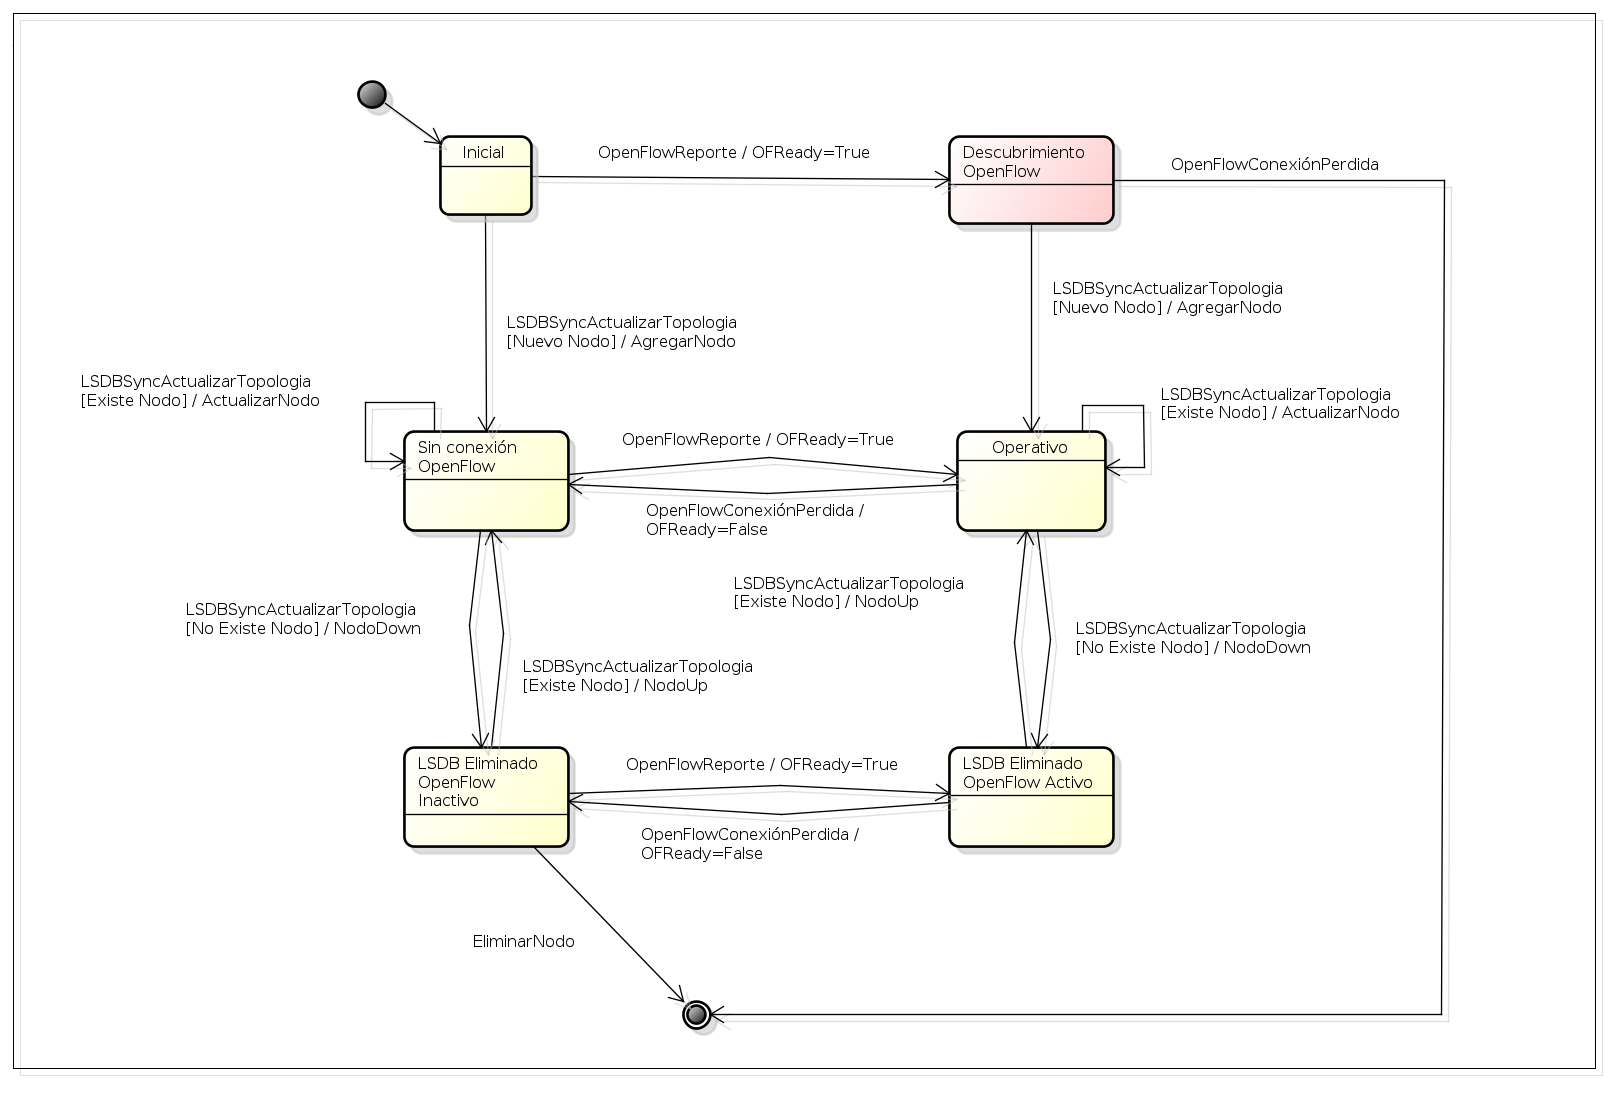
\includegraphics[width=1\textwidth]{CicloVidaNodo2}
\caption[Ciclo de vida de un Nodo]{Ciclo de vida de un Nodo}
\label{fig:CicloVidaNodo}
\end{figure}
  
Como se muestra en la figura\ref{fig:CicloVidaNodo}, descartando el pseudo-estado inicial se identifican cinco estados diferentes para un Nodo: \textit{Descubrimiento OpenFlow}, \textit{Sin Conexión OpenFlow}, \textit{Operativo}, \textit{LSDB Eliminado OpenFlow Inactivo} y \textit{LSDB Eliminado OpenFlow Activo}.\\

El significado de cada uno de estos as\'i como las transiciones posibles se explican a continuación:

\begin{itemize}
\item \textit{Descubrimiento OpenFlow:} Cuando un switch se reporta mediante el canal OpenFlow por primera vez con RAUFlow, se guarda diferente informaci\'on del mismo entre la cual se encuentra la instancia de la clase Datapath en la implementaci\'on de Ryu(esta instancia es utilizada posteriormente para interactuar con el dispositivo). Si el switch OpenFlow no se encuentra instanciado en el sistema como Nodo, la informaci\'on recibida se almacena en una lista auxilar de nodos. No se crea una instancia de Nodo como tal a\'un, instanciandose solamente cuando se advierte la precencia de \'este en la Link State Database(LSDB). 

Esto se corresponde con una decisión de diseño, en la cual se busca reconocer a un Nodo tanto para las funcionalidades de la interfaz gr\'afica de RAUFlow como para el algoritmo de ruteo, solamente cuando se advierte la existencia del mismo en la inforamci\'on de la LSDB. 

De este estado existen dos transiciones posibles. En primer lugar el switch puede dejar de reportarse con el controlador en cuyo caso es eliminado de la lista temporal de nodos y en segundo lugar la componente LSDBSync puede enviar una actualizaci\'on de la topolog\'ia, en donde se incluye el nodo en cuestión. En este caso se instancia un objeto Nodo con toda la informaci\'on provista por la LSDB, datapath de OpenFlow y la inormaci\'on adicional obtenida con el agente SNMP. Luego el Nodo cambia al estado \textit{Operativo}.

Vale la pena destacar que en caso de no poder obtener la informaci\'on adicional con el agente SNMP, el Nodo no es instanciado y se mantiene en el estado actual.

\item \textit{Operacional:}

Este estado es utilizado para representar a aquellos nodos que por un lado se encuentran en la LSDB y fueron rectificados o instanciados en la \'ultima actualizaci\'on de la topolog\'ia, y por otro se encuentran report\'andose mediante el protocolo OpenFlow.

En este estado el nodo es mostrado por la interfaz gr\'afica de RAUFlow y se tiene acceso a todas las características del mismo, tanto del modelo de datos como las que son accesibles a trav\'es del datapath OpenFlow. Adem\'as es considerado para el calculo de las mejores rutas y puede ser utilizado como nodo de ingreso \'o egreso en la definici\'on de servicios.

En pocas palabras es un nodo completamente funcional a los efectos de la implementaci\'on de RAUFlow.

Desde este estado se tienen tres transiciones posibles. Una primera posibilidad es que se produzca una actualización de la LSDB(evento LSDBSyncActualizarTopologia) y que en la topolog\'ia recibida se encuentre el Nodo en cuesti\'on. En este caso solamente se actualiza la informaci\'on asociada al nodo(acción ActualizarNodo), entre la cual se incluye la actualización de las Interfaces y Links, quedando en el estado actual. Una segunda posibilidad es que el switch asociado deje de reportarse por el canal OpenFlow(evento OpenFlowConexiónPerdida) en cuyo caso se modifica el atributo \textbf{of\_ready} del Nodo asignando el valor False y se cambia al estado \textit{Sin Conexión OpenFlow}. Por \'ultimo una tercera posibilidad es que se produzca una actualizaci\'on de la LSDB(evento LSDBSyncActualizarTopologia) y que el Nodo no este en la topolog\'ia recibida. En este caso se deshabilita el Nodo(NodoDOWN) asignando el valor DOWN al atributo \textbf{state} y se cambia al estado \textit{LSDB Eliminado OpenFlow Activo}.

\item \textit{LSDB Eliminado OpenFlow Activo:} Este estado contempla a un Nodo que no se encontraba en la LSDB recibida en la ultima actualizaci\'on topol\'ogica pero que a\'un se reportan por el canal de comunicaci\'on OpenFlow.

Desde este estado se tienen solamente dos transiciones posibles. Una primera posibilidad es que se produzca nuevamente una actualización de la topolog\'ia 
(LSDBSyncActualizarTopologia) y que el nodo se encuentre dentro de la información recibida. En este caso se actualiza el atributo \textbf{state} del nodo valor UP y se cambia al estado \textit{Operativo}. Una segunda posibilidad es que el nodo deje de reportarse por el canal OpenFlow(OpenFlowConexiónPerdida) en cuyo caso se actualiza el valor del atributo \textbf{of\_ready} al valor False y se cambia al estado \textit{LSDB Eliminado OpenFlow Inactivo}.

\item \textit{Sin Conexión OpenFlow:} Este estado contempla a un Nodo que fue creado o rectificado en la \'ultima actualización de la LSDB pero que no se ha reportado por el canal OpenFlow, ya sea porque nunca lo hizo o porque dejo de hacerlo. En este estado el Nodo es mostrado a trav\'es de la interfaz gr\'afica de RAUFlow pero no es considerado ni para el el calculo de mejores caminos ni para la creaci\'on de nuevos servicios tanto como nodo de ingreso \'o como nodo de egreso. Adem\'as la informaci\'on asociada al datapath de OpenFlow como las tabla de flujos y estad\'isticas tampoco son accesibles.

De este estado existen tres transiciones posibles. Por un lado el nodo puede estar presente en la LSDB al producirse una actualizaci\'on de la topolog\'ia\\ (LSDBSyncActualizarTopologia), actualizandose la informaci\'on del nodo \\ (ActualizarNodo) y manteniéndose en el mismo estado. Por otro lado tambi\'en al producirse una actualizaci\'on de la topolog\'ia, el nodo puede no estar en la LSDB, en cuyo caso se actualiza el atributo \textbf{state} al valor DOWN y se cambia al estado \textit{LSDB Eliminado OpenFlow Inactivo}. Finalmente el switch puede empezar a reportarse por el canal OpenFlow(OpenFlowReport) en cuyo caso se actualiza el valor del atributo \textbf{of\_ready} a True y se cambia al estado \textit{Operativo}.  

\item \textit{LSDB Eliminado OpenFlow Inactivo:} Este estado modela a un Nodo que nunca se reporto \'o dej\'o de reportarse por el canal OpenFlow, y que a su vez no se encuentra dentro de la LSDB en la \'ultima actualizaci\'on topol\'ogica realizada. De este estado existen tres transiciones posibles.

Una primera alternativa es que el switch en cuesti\'on se reporte con la aplicaci\'on \\ (OpenFlowReporte), en cuyo caso se actualiza el valor del atributo \textbf{of\_ready} a True y se cambia el estado a \textit{LSDB Eliminado OpenFlow Activo}. Una segunda alternativa es que se produzca una actualizaci\'on de la topolog\'ia y el Nodo se encuentre dentro de la LSDB, en cuyo caso se cambia el valor del atributo \textbf{state} a UP y se cambia al estado \textit{Sin conexión OpenFlow}. Finalmente una tercera alternativa es que el nodo  sea eliminado del sistema. Si bien esta funcionalidad no se encuentra actualmente implementada, la idea es que un Nodo para el cual no se ha recibido reportes por el canal OpenFlow luego de un tiempo determinado, y que tampoco aparece en la LSDB tras una actualicaci\'on, pueda ser eliminado del sistema, eventualmente tras la intervenci\'on de un usuario administrador.
  
\end{itemize}

El ciclo de vida de una Interfaz \'o un Link puede ser explicado de forma an\'aloga con una m\'aquina de estados similar, teniendo presente las relaciones existentes entre las tres clases, Nodos, Interfaces y Links.\\ \\

De esta forma queda explicada la implementaci\'on de la aplicaci\'on de gesti\'on RAUFlow, el diseño de  los nodos que formar\'an parte de la red prototipo (RAU-Switch) y el funcionamiento general del prototipo en su conjunto. 

El siguiente cap\'itulo esta destinado al diseño y construcción de un laboratorio de pruebas, para la validaci\'on de las componentes desarrolladas y la implementaci\'on de algunos casos de uso representativos. 





